\documentclass[a4paper,12pt]{article}

\usepackage[utf8]{inputenc}
\usepackage[T1]{fontenc}
\usepackage{amsmath,amssymb,amsfonts}
\usepackage{graphicx}
\usepackage[margin=20mm]{geometry}
\usepackage{color}

\newcommand{\todo}[1]{{\color{blue} TODO[#1]}}

\begin{document}

\title{5DV152/VT15: Lab 5}
\author{Christer Jakobsson (870310-8533)}
\date{\today}
\maketitle
  

\section{Study technique}

I studied the article in the way that i first read the sections in the paper in the order told from the assignment page.
Afterwards i slowly re-read the parts that i didn't understand and tried to fathom what where told.
Then i started to explore how hash join and merge-sort join works, so that i had basic understanding of how they worked sequentially.
I enhanced my understanding by using google to read explanations of the both join methods and youtube to watch videos to understand well.
\\\\
I have discussed alot with some of my study mates that also takes the course and this feels like the most rewarding way of understanding, having the opportunity to discuss with others how they understand the article and its content.
\\
After getting more knowledge about the two methods i then carefully read the parts i am supposed to explain in this report, step by step going through each part to try and understand whats happening in each part.

\section{Explanation of Steps P1-P3}
\label{sec:exp}

\begin{itemize}
 \item \emph{P1:} The first step in the parallel partitioning phase, evenly splits the tuples so they fit in the L2 cache and submit them to tasks, which will be executed by the systems cores. Each task builds a local histogram and iterates over each tuple and updates it using a defined hash function.
 \item \emph{P2:} Compute the prefix sum for each tuple in parallel. The prefix sum is used to calculate where the offset for each tuple should be in a merged histogram, using the prefix sum for displacement of the tuples. 
 \item \emph{P3:} Each task moves all its tuples to the their final destination, a histogram structure, which offset was calculated in P2.
\end{itemize}

\subsection{Small example}
I will use an example with one database table that holds names and an id and one that holds telephone numbers and an id. There will be two threads used.
\newpage

\textbf{NameTable}\\
\begin{tabular}{| r | c | r |}
\hline
Key & Name \\ \hline
1 & Bob \\ \hline
2 & Alice \\ \hline
3 & Jane \\ \hline
4 & George \\ \hline
\hline
\end{tabular}
\\\\
\textbf{TelephoneTable}\\
\begin{tabular}{| r | c | r |}
\hline
Key & Name \\ \hline
1 & 123 \\ \hline
1 & 322 \\ \hline
2 & 456 \\ \hline
2 & 543 \\ \hline
3 & 789 \\ \hline
3 & 987 \\ \hline
4 & 957 \\ \hline
4 & 593 \\ \hline
\hline
\end{tabular}
\\\\
If i then want to find the telephone numbers for several names,  the outer relation will be NameTable (S) and the inner relation will be TelehponeNumber (R). 
\\\\
Then S will be split into tasks that will fit into the cache, in this example i will say that each task can hold two tuples, so the first task will consist of Bob and Alice
and the second will contain Jane and George.
\\\\
Then the prefix sum for each tuple are computed to know where each tuple should start in the histogram, and then all tuples get moved to their destination in the histogram.\\

\section{The three phases of the parallelized join}

Tasks are created, same amount as there is outer sub-tables from steps P1 - P3. If the inner-table and outer-table that the join operations is supposed to be done on is smaller than a pre defined threshold the join operation is performed on the tables.
The result from the join gets added to the output table, in the event where any of the two tables is bigger then the threshold the table-pair is added to a list of pairs that will be addressed in the next phase.
There is explicit barrier at the end of the first phase, which syncronizes the threads for the next phase.
\\\\
The outer-tables gets split into smaller tables that can reside in the cache in a parallel, and all keys that are going to be probed gets put in a list. 
After this has been done all threads starts to go through the list of keys and searches for mathing keys and adds the appropriate tuples to their output tables.
\\\\
Motivation behind each phase:
\begin{itemize}
 \item \emph{Phase 1:} This step is used to check if outer-table (S) is already small enough to fit into the L2 cache and if it is the join is made here and dont need to go through phase 2-3. Acts as a initial check, if the tables are small enough phase 2-3 wont be executed.
 \item \emph{Phase 2:} Used to split the inner relation into smaller pieces in the same manner as in \ref{sec:exp} but on the inner relation, puts the keys into a list to be used in phase 3.
 \item \emph{Phase 3:} Threads search for matching keys in both inner and outer tables and on a match puts the tuples in their output table.
\end{itemize}

\section{The bandwidth-oblivious sort}
The bandwidth oblivious sort works so that a tree of threads are created, the lists are split up until there is two tuples in each list.
Then the leaf nodes all sorts their lists in parallel, then they start to send the head of their list up until their parent, which also is a thread.
Then that parent has a list of two tuples, and in turn sends its lists head up to its parent, this goes on until all tuples have reached the root node.
The node then holds a sorted list of all tuples which then get written to memory.
\\\\
The purpose of doing it in this way is that by only sending one tuple at a time it will not be written to disk to send it to another core. If the leaf nodes where to send their whole list, containing two tuples, that 
would not fit into the L2 Cache so the operation would need to write and read from memory. 
The end result is that all operations to merge all small lists into a list with all tuples, are utilzing the cache and only the tuples are only written and read once, which is more efficient than having to read/write from memory.

\newpage

\subsection{Illustrative picture}
In the Figure \ref{fig:flock-pic} the starting list is [1,5,2,4,3,7,6,8] and it gets split, each leaf sorts its list first. Then each leaf sends its head to its parent, and that parent will sort its incoming  keys and send the head of that list to its parent.
This will then repeat until the root have the sorted list. The main thing with the method is to only send the head of the list and not the whole list to the parent, since the head (tuple) cfit in the cache.

\begin{figure}[h!]
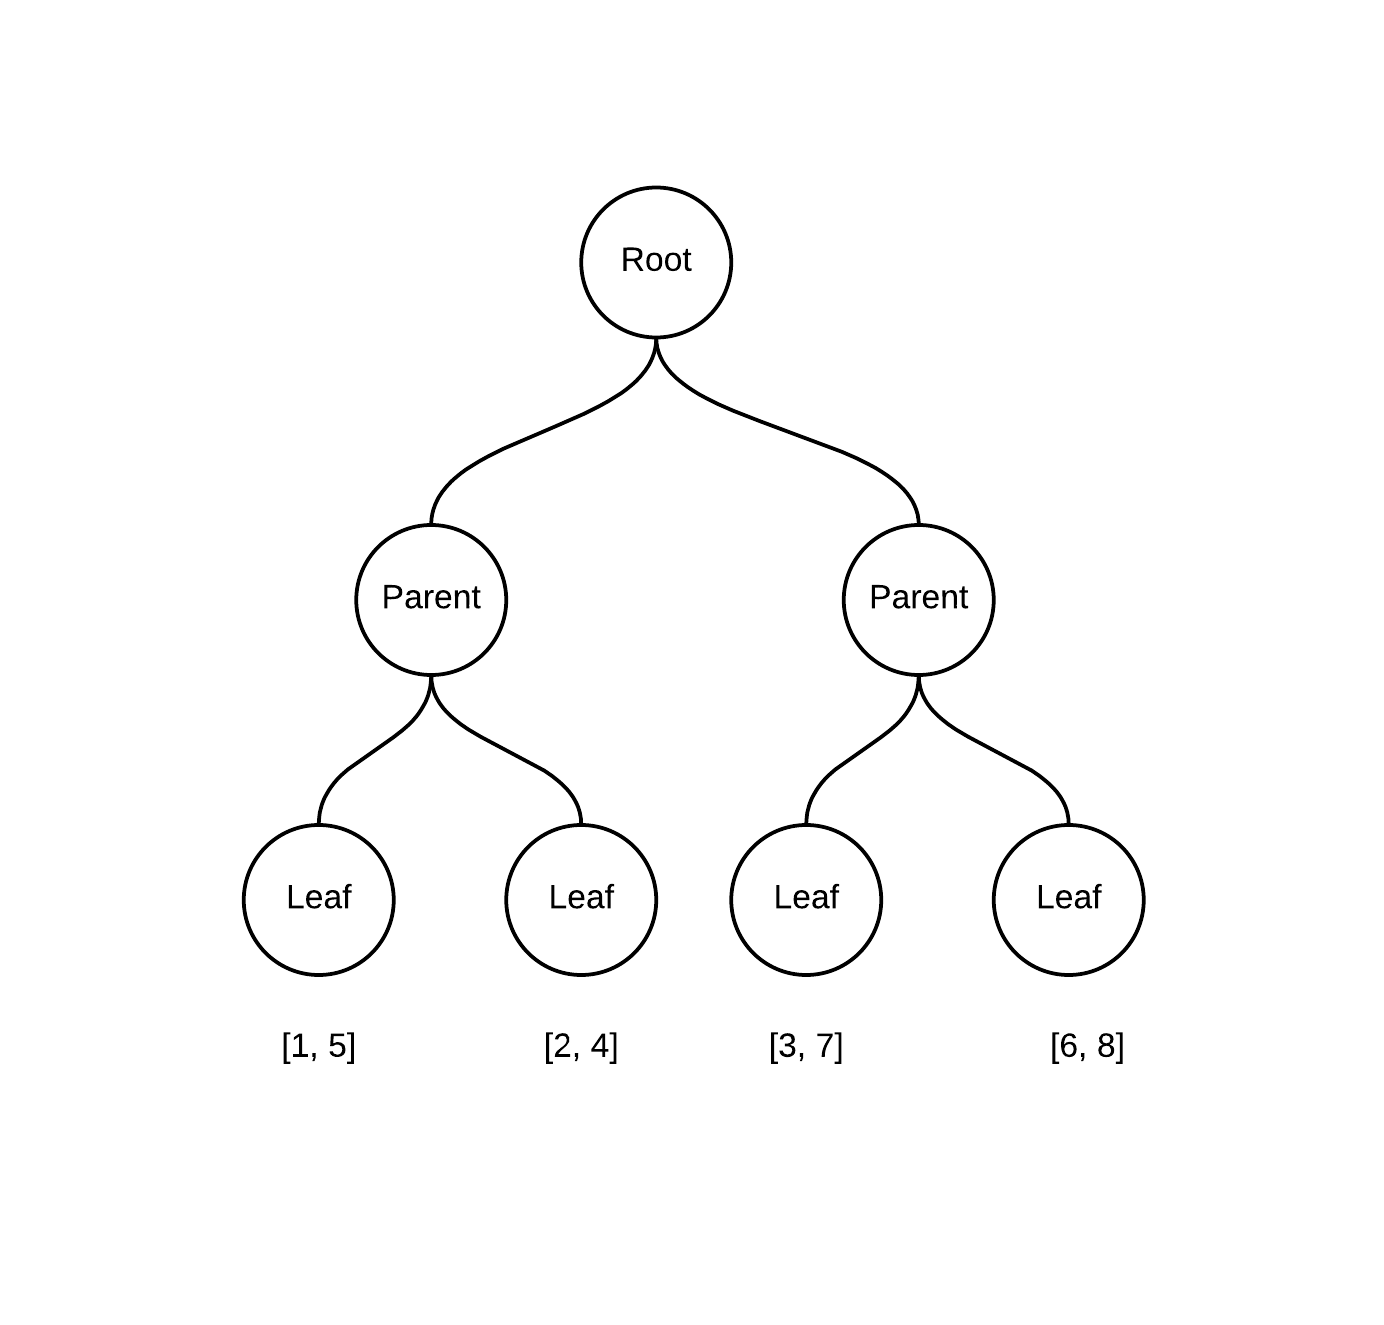
\includegraphics{bandwidth-oblivious-sort}
\caption{\emph{Bandwidth-oblivious-sort}}
\label{fig:flock-pic}
\end{figure}

\section{Reflection}

I feel that i have learned much both in terms of what this course is about (Parallel programming) and how to study a scientific reports contents and understand it.
I have not taken a course in learning databases so my prior knowledge about databases us quite basic, this have been one small obstacle since i needed to learn what a \emph{join} was.
I feel that i have learned much from this lab, i have learned more about how one can go through to make a parallelisation of something sequential and what obstacles there is when doing it,
and also that the technic used to parallelize can give very different results in effectivity
\\\\
To study the article in depth i felt that i needed time. Read the whole article, come back the next day read the hard parts again, i feel that the main challange for me to complete this assignment is time.
\\\\
I did not have opportunity to participate in the seminar.

\begin{itemize}
\item Reflect on your learning experience in this lab.
\item What was it like to study the article in depth? What was the main challenge for you? 
\item How did your participation in the seminar affect your understanding of the article?
\item What did you learn while writing this report?
\end{itemize}

\end{document}